% =============================================================================
% ICLR 2027 COLLABORATIVE MANUSCRIPT
% =============================================================================
% Overleaf setup:
%   1. Upload this file together with iclr2027_conference.sty,
%      iclr2027_conference.bst, and OVERLEAF_ICLR2027_REFERENCES.bib.
%   2. Set this file as the Overleaf Main document.
%   3. Keep \iclrfinalcopy commented for anonymous submission.
%
% Collaboration workflow:
%   - Visible draft annotations are ON by default.
%   - Before any submission build, switch \showcommentstrue to
%     \showcommentsfalse and search the source for TODO, CHECK, and CLAIM.
%   - Source comments beginning with CLAIM STATUS record the evidence ceiling.
%   - Do not add results without a seed-level record and a frozen metric label.
%
% CLAIM STATUS (current):
%   [EXACT]      One-sided product structure, factorial identities, shared-RNG
%                trajectory recursion, and stage-0 q/g reparameterization.
%   [FORMAL]     Seeds 3--5, q=256, 256 kimg factorial and 256--1024 curves.
%   [SECONDARY]  Seeds 14--18 learning-curve sensitivity analysis.
%   [SUPPORTING] Frozen-state RAdam virtual-update diagnostics.
%   [PENDING]    Prospectively unseen cohort, AUC/time-to-quality primary test,
%                and second weighting rule.
% =============================================================================

\documentclass{article}
\usepackage{iclr2027_conference,times}

\usepackage{amsmath,amssymb,amsthm,mathtools,bm}
\usepackage{booktabs}
\usepackage{graphicx}
\usepackage{xcolor}
\usepackage{hyperref}
\usepackage{url}

% -----------------------------------------------------------------------------
% Collaboration annotations. These must be disabled for submission.
% -----------------------------------------------------------------------------
\newif\ifshowcomments
\showcommentstrue
% \showcommentsfalse

\definecolor{todored}{RGB}{180,35,35}
\definecolor{theoryblue}{RGB}{25,85,160}
\definecolor{empiricalgreen}{RGB}{20,120,80}
\definecolor{claimpurple}{RGB}{110,55,145}

\newcommand{\todo}[1]{%
  \ifshowcomments{\color{todored}\textbf{[TODO: #1]}}\fi}
\newcommand{\theorynote}[1]{%
  \ifshowcomments{\color{theoryblue}\textbf{[THEORY CHECK: #1]}}\fi}
\newcommand{\empnote}[1]{%
  \ifshowcomments{\color{empiricalgreen}\textbf{[EMPIRICAL CHECK: #1]}}\fi}
\newcommand{\claimnote}[1]{%
  \ifshowcomments{\color{claimpurple}\textbf{[CLAIM CEILING: #1]}}\fi}

\newcommand{\sg}{\operatorname{sg}}
\newcommand{\Dsg}{\mathcal{D}^{\mathrm{sg}}_\theta}
\newcommand{\Ropt}{R_{\mathrm{opt}}}

\newtheorem{proposition}{Proposition}
\newtheorem{lemma}{Lemma}

% COLLAB NOTE (claim ceiling): keep the title ECT- and pair-spacing-specific
% unless a prospectively frozen cohort and a second weighting regime support
% the broader ``optimization geometry of consistency gaps'' framing.
\title{ECT Pair Spacing: Exact Decomposition\\and Finite-Training Dynamics}

% Authors are hidden by the ICLR style while \iclrfinalcopy is commented.
\author{Anonymous Authors}

% \iclrfinalcopy % Uncomment only for the accepted camera-ready version.

\begin{document}

\maketitle

\begin{abstract}
Prior work shows that consistency discretization changes convergence speed.
We characterize the narrower intervention induced by changing the realized
spacing of an ECT training pair. In the evaluated stage-0, unclipped protocol,
the $g=1.10$ rule is, at pair construction, exactly the
$q_{\mathrm{eff}}=256/1.10\simeq232.727$ rule. Our theoretical object is
therefore realized spacing rather than a distinct $g$ mechanism. At a
fixed model state and stochastic realization, its one-sided stop-gradient
training derivative admits, under the stated regularity conditions, an exact
weight-first decomposition into explicit reweighting and detached-target
endpoint displacement; the target-first path has the same total but reallocates
the interaction. A matched four-cell cross-assignment diagnostic
obeys exact common-state scaling identities, while a two-step SGD construction
shows that these identities do not determine the parameter factorial contrast
formed after separate training. In the formal three-seed experiment, the
observed preregistered 256-kimg NFE1 FID contrast for the complete spacing
intervention is favorable in every seed, while denominator and
factorial-interaction contrasts vary in direction. Budget-resolved evaluation
from 256 to 1024 kimg shows large early differences followed by smaller,
seed-dependent contrasts and changing arm rankings. In a five-seed secondary
cohort, the descriptive 1024-kimg
cohort-mean minima occur in different arms under NFE1 and NFE2. The results
distinguish an exact common-state intervention structure from its
trajectory-dependent finite-training consequences.
\end{abstract}

\todo{Abstract: re-check wording after the prospectively unseen cohort is
complete; do not replace the current evidence status before unblinding.}

\section{Introduction}
\label{sec:introduction}

Consistency models support one- or few-step generation by learning a mapping
that is consistent along a noise trajectory \citep{song2023consistency}.
Easy Consistency Tuning (ECT) constructs paired states at different times and
trains an online prediction against a detached target
\citep{geng2024consistency}. Their temporal separation---called the
\emph{consistency gap} in this paper---can change early FID and KID even when,
under strong ideal assumptions,
feasible zero-edge solutions agree on boundary-determined values over common
reachable latent support. We ask why pair spacing can nevertheless alter
finite-budget learning speed and quality.

We study the realized spacing $\Delta=t-r$ conditional on the baseline
$q=256$ schedule. In the evaluated single-stage, unclipped window, the
$g=1.10$ pair rule is exactly the
$q_{\mathrm{eff}}=256/1.10\simeq232.727$ pair rule for every sampled $t$.
Thus the experiment studies a spacing intervention, not a distinct
$g$-specific mechanism. In the inverse-spacing ECT objective, changing
$\Delta$ jointly changes the detached target endpoint and explicit loss
weight. We derive their exact common-state relations and test what remains
after the arms enter separate parameter and optimizer trajectories.

Our contributions are:
\begin{enumerate}
  \item \textbf{Controlled cross-assignment construction and exact common-state
  identities.}
  We define the one-sided stop-gradient derivative and a four-cell
  target-by-weight diagnostic whose cross-assigned cells are off-family
  diagnostic probes. The resulting product structure separates explicit
  reweighting from detached-endpoint displacement under general
  parameter-independent weights.

  \item \textbf{Finite-trajectory implication boundary.}
  An exact shared-RNG SGD recurrence separates the matched-state factorial
  term from state-divergence feedback. A two-step construction shows that
  global common-state identities need not yield a zero parameter factorial
  contrast after separate training.

  \item \textbf{Budget-resolved evidence.}
  At 256 kimg, target-related NFE1 contrasts favor the enlarged endpoint in
  all three formal seeds, whereas denominator and interaction contrasts vary
  in direction. Within those seeds, seven-budget differences contract and arm
  rankings vary with seed and sampling NFE; a secondary five-seed cohort
  separately exhibits different descriptive long-budget minima across NFE.
\end{enumerate}

\claimnote{Keep the novelty boundary at the controlled cross-assignment construction,
exact common-state identities, and the finite-trajectory implication boundary.
The chain-rule product identity is algebraic infrastructure, not a standalone
deep theorem. Do not re-center the narrative on RAdam history, balanced beta,
optimizer scale invariance, or a universal best gap.}

\section{Relation to discretization, curricula, and weighting}
\label{sec:related-work}

Consistency-model objectives expose both a discretization schedule and a loss
weight \citep{song2023consistency}. Improved consistency training changes the
curriculum and uses inverse-spacing weights \citep{song2024improved}; ECT uses
a continuous pair mapping and shrinks its spacing through $q$. After observing
that $1/(t-r)$ couples mapping and weight, ECT explicitly evaluates decoupled
weighting alternatives \citep{geng2024consistency}.
These works also document finite-budget tradeoffs across discretizations and
curricula, making pair spacing, weighting, and convergence speed established
parts of consistency-model design.

Truncated Consistency Models analyzes a stopped-target objective with an
explicit $\omega(t)/\Delta_t$ factor \citep{lee2025truncated}; Stable
Consistency Tuning relates pair spacing to bootstrapped error propagation
\citep{wang2024stable}. Consistent Diffusion Language Models separates
step-size and weight schedulers while retaining an inverse-step weight and
stopped target \citep{amin2026consistent}. Related work develops
continuous-time objectives, discretization-complexity analyses, jointly
adaptive discretization and weighting, and flow-map or self-distillation
formulations \citep{lu2024simplifying,yang2025discretization,bai2025adaptive,
boffi2025flowmap,boffi2025how}; complementary theory studies convergence and
stop-gradient stability \citep{li2025theory,kim2026stabilizing}.
A concurrent modular study deconstructs the broader training pipeline into time
discretization, preconditioning, weighting, and sampling
\citep{anonymous2026guide}.
Recent work studies consistency-model training geometry through output-time
tangent alignment \citep{kim2025align}; another uses ``consistency gap'' for the
distinct discrepancy between a teacher denoiser and an optimal student
denoiser \citep{zheng2025preconditioning}. Here \emph{gap} means temporal pair
spacing, and our geometry is the common-state parameter training field.

Our narrower contribution is a controlled, cross-assigned target-by-weight
factorial for finite-spacing one-sided-SG ECT, exact common-state identities,
and the implication boundary to factorial contrasts formed after separate
training. The chain-rule product identity serves as algebraic infrastructure
for this design, rather than as a new general theory of discretization.

\section{Consistency gaps as composite interventions}
\label{sec:theory}

\paragraph{The roles of $q$, $g$, and realized pair spacing.}

Let $j\in\{0,1,\ldots\}$ index the ECT curriculum stage and define
$n(t)=1+k\,\sigma(-bt)$. Under the repository convention, the official
sigmoid mapping and its realized spacing are
\begin{equation}
  r_q(t,j)=\max\!\left\{0,
    t\left(1-\frac{n(t)}{q^{j+1}}\right)\right\},
  \qquad
  \Delta_q(t,j)=t-r_q(t,j)
  =\min\!\left\{t,\frac{t\,n(t)}{q^{j+1}}\right\}.
  \label{eq:q-realized-spacing}
\end{equation}
The global probe $g>0$ acts on this realized baseline spacing through the
production clamp,
\begin{equation}
  \Delta_{q,g}(t,j)=\min\{t,g\Delta_q(t,j)\},
  \qquad r_{q,g}(t,j)=t-\Delta_{q,g}(t,j).
  \label{eq:g-realized-spacing}
\end{equation}
Thus $q$ and $g$ both parameterize the realized pair. Conditional on a fixed
stage and away from clipping, a
$g$-scaled pair can be written as a stage-specific effective value
$q_{\mathrm{eff}}(j)=q/g^{1/(j+1)}$. A single fixed $q_{\mathrm{eff}}$ does not
generally reproduce the same constant-$g$ perturbation across multiple stages,
and clipping must be checked on the realized pairs.

The formal protocol has $q=256$, $k=8$, $b=1$, $g=1.10$, and
\texttt{double\_ticks}=10000 with 10 kimg per tick. Its entire 1024-kimg
horizon therefore remains at $j=0$.
For $t\geq0$, $n(t)=1+8\sigma(-t)\leq5$, so
$g n(t)/q\leq5.5/256<1$ and neither pair rule clips. Hence, pointwise in $t$,
\begin{equation}
  \Delta_{256,1.10}(t,0)
  =\Delta_{256/1.10,1}(t,0),
  \qquad q_{\mathrm{eff}}=256/1.10\simeq232.727.
  \label{eq:q-g-exact-reparameterization}
\end{equation}
This establishes the same theoretical pair-spacing rule in real arithmetic.
A matched-$q$ control would test whether the implementation and floating-point
paths preserve it; Equation~\eqref{eq:q-g-exact-reparameterization} alone does
not prove full training-code equivalence.

The effective spacing of a training design is consequently the joint law of
$(J,T,\Delta_{q,g}(T,J))$ under its frozen stage curriculum and time sampler,
not one scalar hyperparameter or a cohort-average gap. We use the native ECT
coordinate $\Delta=t-r$ because it determines both the detached target at $r$
and the explicit denominator in the CIFAR-10 objective. The current experiment
holds $q=256$ fixed and uses $g$ only as a controlled probe of this pair-spacing
intervention.

\claimnote{Describe $g$ as a controlled implementation probe of pair spacing.
In this protocol it is exactly a stage-0 $q_{\mathrm{eff}}$
reparameterization at pair construction.}

\subsection{Ideal target and endpoint-invariance intuition}
\label{sec:theory-ideal-endpoint}

Let $\gamma_\omega(t)$ denote a latent coupled trajectory with anchor time
$t_\star$. A schedule is \emph{anchor-reaching} on the relevant support if,
from every supported $(\omega,t_0)$, its legal edges generate a decreasing
sequence $t_0>t_1>\cdots$ that either reaches $t_\star$ in finitely many steps
or converges to it.

\begin{lemma}[Ideal endpoint invariance]
\label{lem:ideal-endpoint-invariance}
Let $S\in\{S_1,S_2\}$ index two anchor-reaching schedules, each admitting at
least one feasible ideal solution. Suppose that:
\begin{enumerate}
  \item both schedules use the same latent trajectories and common anchor;
  \item for each $S$, any feasible ideal solution $F_S^\star$ satisfies the
  pointwise edge equalities on every legal path,
  $F_S^\star(\gamma_\omega(t_m),t_m)
   =F_S^\star(\gamma_\omega(t_{m+1}),t_{m+1})$;
  \item $F_S^\star(\gamma_\omega(t),t)$ is continuous at $t_\star$ along every
  infinite legal path; and
  \item every solution has the common boundary value
  $F_S^\star(\gamma_\omega(t_\star),t_\star)
   =b(\gamma_\omega(t_\star))$.
\end{enumerate}
Then, for each $S\in\{S_1,S_2\}$, every feasible ideal solution satisfies,
on $S$'s reachable support,
\begin{equation}
  F_S^\star(\gamma_\omega(t),t)
  =b(\gamma_\omega(t_\star)).
  \label{eq:ideal-endpoint-invariance}
\end{equation}
Hence, at every common latent-indexed point $(\omega,t)$ reachable under both
schedules, their feasible ideal solutions take the same boundary-determined
value.
\end{lemma}

This lemma formalizes the endpoint intuition under trajectory-compatible zero
edge constraints. For the formal stage-0 rule with $t_\star=0$,
$n(t)\geq1$ implies $t_{m+1}\leq(1-q^{-1})t_m$, so repeated endpoints approach
the anchor even when they do not reach it finitely. The shared-noise ECT line
$\gamma_{y,\varepsilon}(t)=y+t\varepsilon$ supplies a coupling, but zero
residual across every latent line is a feasibility assumption: different
latent lines can impose incompatible values at the same observed $(x,t)$.
Thus Lemma~\ref{lem:ideal-endpoint-invariance} is a conditional endpoint-invariance
statement, not a characterization of a finite-capacity ECT population
minimizer.

Connecting the pointwise premise to a population risk requires additional
measure conditions: positive edge weights, a nonnegative penalty that vanishes
only at zero residual, and enough support and continuity to extend an
almost-everywhere equality. We use the lemma only after stating its pointwise
ideal premise.

\theorynote{Keep the lemma on latent trajectories and retain the asymptotic
anchor case. Do not silently upgrade feasibility of zero pathwise residuals
into a property of the actual ECT population minimizer.}

\subsection{Exact ECT composite intervention}
\label{sec:theory-composite-intervention}

The preceding ideal invariance does not make the finite-training intervention
scalar. Fix one stochastic realization $\zeta$, including data, time, noise,
augmentation, dropout masks, and schedule state. Let
$x_t=y+t\varepsilon$, $x_r=y+r\varepsilon$, and define
\begin{equation}
  D_\theta=f_\theta(x_t,t),\qquad
  T_{\bar\theta,r}=f_{\bar\theta}(x_r,r),\qquad
  e_r(\theta)=D_\theta-
  \left.T_{\bar\theta,r}\right|_{\bar\theta=\theta}.
  \label{eq:ect-residual}
\end{equation}
For an explicit finite positive weight $w_r=w(t,r;\zeta)$ and a residual
penalty $\varphi$, introduce the lifted loss
\begin{equation}
  \widetilde\ell_{r,w}(\theta,\bar\theta;\zeta)
  :=w_r\,\varphi\!\left(D_\theta-T_{\bar\theta,r}\right),
  \qquad
  \ell_{r,w}(\theta;\zeta)
  :=\widetilde\ell_{r,w}(\theta,\theta;\zeta),
  \qquad
  \Dsg\ell_{r,w}
  :=\left.\nabla_\theta\widetilde\ell_{r,w}
  \right|_{\bar\theta=\theta}.
  \label{eq:sg-training-derivative}
\end{equation}
The endpoint, weight, and $\zeta$ are held fixed during backpropagation, with
$\nabla_\theta w_r=\nabla_{\bar\theta}w_r=0$. This derivative preserves the
target's forward value while suppressing its parameter derivative. When both
partial derivatives exist, it differs from the ordinary diagonal derivative,
which contains both $\nabla_\theta\widetilde\ell$ and
$\nabla_{\bar\theta}\widetilde\ell$.

\begin{proposition}[Exact common-state one-sided product structure]
\label{prop:sg-product-structure}
Let $\theta\in\mathbb{R}^p$, let the residual lie in $\mathbb{R}^d$, and let
$\varphi:\mathbb{R}^d\to\mathbb{R}$. Assume $\theta\mapsto D_\theta$ and
$\varphi$ are differentiable at the realized state and residuals,
respectively. Define
\begin{equation}
  J_t:=\frac{\partial D_\theta}{\partial\theta}
    \in\mathbb{R}^{d\times p},
  \qquad
  v_r:=\nabla_e\varphi(e_r),
  \qquad
  H_r:=J_t^\top v_r.
  \label{eq:sg-unweighted-field}
\end{equation}
Then the one-sided SG training field is exactly
\begin{equation}
  G_{r,w}^{\mathrm{sg}}(\theta;\zeta)
  :=\Dsg\ell_{r,w}=w_r H_r.
  \label{eq:sg-product-structure}
\end{equation}
For endpoints $r_1,r_g$ and parameter-independent weights $w_1,w_g$, let
$\alpha:=w_g/w_1$ and, for $a\in\{1,g\}$, define
$\ell_a:=\widetilde\ell_{r_a,w_a}(\theta,\theta;\zeta)$ and
$G_a^{\mathrm{sg}}:=G_{r_a,w_a}^{\mathrm{sg}}(\theta;\zeta)$.
The complete intervention satisfies
\begin{align}
  \ell_g
  &=\alpha\ell_1
    +w_g\!\left[\varphi(e_{r_g})-\varphi(e_{r_1})\right],
  \label{eq:general-loss-decomposition}\\
  G_g^{\mathrm{sg}}
  &=\alpha G_1^{\mathrm{sg}}
    +w_gJ_t^\top(v_{r_g}-v_{r_1}).
  \label{eq:general-weight-decomposition}
\end{align}
\end{proposition}

For any realized sample in the formal ECT setting with
$\Delta_1,\Delta_g>0$ and $e_{r_1},e_{r_g}\neq0$, we have
$\varphi(e)=\lVert e\rVert_2$ and $w_r=1/\Delta_r$. Hence
$v_r=u_r:=e_r/\lVert e_r\rVert_2$ and
$\alpha=\Delta_1/\Delta_g=:s$. Proposition~\ref{prop:sg-product-structure}
specializes to
\begin{align}
  \ell_g
  &=s\ell_1
    +\underbrace{\frac{\lVert e_{r_g}\rVert_2
      -\lVert e_{r_1}\rVert_2}{\Delta_g}}
      _{\tau^{(\ell)}_{\mathrm{tar}}},
  \label{eq:exact-ect-loss-decomposition}\\
  G_g^{\mathrm{sg}}
  &=sG_1^{\mathrm{sg}}
    +\underbrace{\frac{1}{\Delta_g}J_t^\top
      \left(u_{r_g}-u_{r_1}\right)}
      _{\tau^{(G)}_{\mathrm{tar}}}.
  \label{eq:exact-ect-gradient-decomposition}
\end{align}

Equivalently, the change relative to the baseline is
\begin{align}
  \ell_g-\ell_1
  &=(s-1)\ell_1+\tau^{(\ell)}_{\mathrm{tar}},
  \label{eq:exact-ect-loss-change}\\
  G_g^{\mathrm{sg}}-G_1^{\mathrm{sg}}
  &=(s-1)G_1^{\mathrm{sg}}+\tau^{(G)}_{\mathrm{tar}}.
  \label{eq:exact-ect-gradient-change}
\end{align}
Thus $s\ell_1$ and $sG_1^{\mathrm{sg}}$ are the
\emph{denominator-rescaled baseline terms} in the post-intervention value,
whereas $(s-1)\ell_1$ and $(s-1)G_1^{\mathrm{sg}}$ are the corresponding
explicit denominator-rescaling changes. The $\tau_{\mathrm{tar}}$ terms are
the target-endpoint displacements along the weight-first path
$A\to D\to B$. A target-first path $A\to C\to B$ gives the same total change
but reallocates the exact factorial interaction between its two components;
neither path defines a causal percentage attribution. Their joint change is
the \emph{ECT composite gap intervention}.
Equations~\eqref{eq:exact-ect-loss-decomposition}--
\eqref{eq:exact-ect-gradient-decomposition} require neither a small-gap
approximation nor an optimizer model. Only the denominator-rescaling component
is represented by an exact scalar multiple of the baseline field. When
$G_1^{\mathrm{sg}}\neq0$, the complete field lies in the span of the baseline
field if and only if its target-endpoint component is collinear with that
field; when $G_1^{\mathrm{sg}}=0$, scalar equivalence requires the complete
field to vanish.
When $G_1^{\mathrm{sg}}\neq0$, the least-squares scalar coefficient of the
complete field against the baseline is
\begin{equation}
  a^\star
  :=\frac{\langle G_g^{\mathrm{sg}},G_1^{\mathrm{sg}}\rangle}
  {\lVert G_1^{\mathrm{sg}}\rVert_2^2}
  =s+
  \frac{\langle\tau^{(G)}_{\mathrm{tar}},G_1^{\mathrm{sg}}\rangle}
  {\lVert G_1^{\mathrm{sg}}\rVert_2^2}.
  \label{eq:best-scalar-mixes-components}
\end{equation}
Thus $a^\star$ mixes the explicit denominator ratio with the projection of
the target displacement; it is not an estimator of $s$ alone. In the general
notation of Equation~\eqref{eq:general-weight-decomposition}, the
explicit ratio is $\alpha$; for the inverse-spacing ECT specialization here,
$\alpha=s=1/g$.

For the formal $c=0$ loss, $\varphi(e)=\lVert e\rVert_2$ is not differentiable
at $e=0$, so Equations~\eqref{eq:exact-ect-gradient-decomposition} and
\eqref{eq:exact-ect-gradient-change} use their stated nonzero-residual
condition. The product and factorial identities extend to selected one-sided
subgradient fields: choose $v_r\in\partial\lVert e_r\rVert_2$ for each endpoint
and use the same $v_r$ whenever that endpoint appears under different weights.
This shared selection is a mathematical condition, not an asserted autograd
convention. The pending real-network $c=0$ audit is fail-closed: an exact zero
residual invalidates the affected audit instance, and no derivative identity is
reported unless the implementation convention is first verified.

\theorynote{Weights not held fixed during the one-sided derivative, including
undetached residual-dependent or learned weights, require additional
derivative terms and are outside
Proposition~\ref{prop:sg-product-structure}. Do not replace the fail-closed
$e=0$ audit rule with an assumed implementation convention.}

\subsection{Exact factorial identities}
\label{sec:theory-factorial-identities}

The product structure yields exact common-state factorial identities. For a
matched sample, define the four cells
\begin{equation}
  A=(r_1,w_1),\qquad
  B=(r_g,w_g),\qquad
  C=(r_g,w_1),\qquad
  D=(r_1,w_g),
  \label{eq:factorial-cells}
\end{equation}
where the first coordinate selects the detached target endpoint and the second
selects the explicit parameter-independent weight. Proposition
\ref{prop:sg-product-structure} gives
\begin{align}
  \ell_B&=\alpha\ell_C,&
  \ell_D&=\alpha\ell_A,&
  \ell_B-\ell_D&=\alpha(\ell_C-\ell_A),
  \label{eq:factorial-loss-identities}\\
  G_B^{\mathrm{sg}}&=\alpha G_C^{\mathrm{sg}},&
  G_D^{\mathrm{sg}}&=\alpha G_A^{\mathrm{sg}},&
  G_B^{\mathrm{sg}}-G_D^{\mathrm{sg}}
  &=\alpha(G_C^{\mathrm{sg}}-G_A^{\mathrm{sg}}).
  \label{eq:factorial-gradient-identities}
\end{align}
The corresponding factorial interactions obey
\begin{align}
  I_\ell:=\ell_B-\ell_C-\ell_D+\ell_A
  &=(\alpha-1)(\ell_C-\ell_A),\\
  I_G:=G_B^{\mathrm{sg}}-G_C^{\mathrm{sg}}
      -G_D^{\mathrm{sg}}+G_A^{\mathrm{sg}}
  &=(\alpha-1)(G_C^{\mathrm{sg}}-G_A^{\mathrm{sg}})
    =(w_g-w_1)(H_{r_g}-H_{r_1}).
  \label{eq:exact-factorial-interactions}
\end{align}
In the inverse-spacing ECT objective, A and B are the two on-manifold cells:
each pairs an endpoint with the weight induced by that same spacing. C and D
deliberately cross-assign these coordinates. They are cross-assigned off-family
diagnostic probes used to characterize the composite intervention, not legal gap
schedules.

\claimnote{Describe C and D as cross-assigned off-family diagnostic probes. Do not present
them as legal independent schedules or as a $q\times g$ factorial.}

The interaction is exactly determined and is generally nonzero. In the
unclipped ECT specialization, $\alpha=s=1/g$ is common to all samples, so the
scaling identities also hold after minibatch aggregation. With clipping,
$s_i=\Delta_{1,i}/\Delta_{g,i}$ can vary across samples: the identities remain
exact per sample, but $s_i$ cannot be pulled outside the minibatch sum.

\emph{These identities exactly characterize the intervention at a common model
state; they neither determine the factorial contrast formed from separately
trained quality outcomes nor make that contrast seed invariant.}
Once the four arms follow separate parameter trajectories, the matched
quantities in Eqs.~\eqref{eq:factorial-loss-identities}--
\eqref{eq:exact-factorial-interactions} are no longer held fixed. The theory
therefore motivates the cross-assignment diagnostic without predetermining its
finite-training quality contrasts.

\section{Formal target-by-denominator diagnostic}
\label{sec:factorial-experiment}

\subsection{Design and estimands}

We probe the decomposition with a $2\times2$ cross-assignment diagnostic in the $q=256$
ECT setting. The enlarged-gap condition uses a global multiplier $g=1.10$.
The design is a target-by-denominator factorial for the realized spacing
intervention conditional on this baseline schedule, not a $q\times g$
factorial. Equation~\eqref{eq:q-g-exact-reparameterization} records the exact
stage-0 $q_{\mathrm{eff}}$ representation of its pair rule.
The four arms are shown in Table~\ref{tab:arms}. Arms share the same starting
checkpoint, data order, sampled times, noise, dropout stream, optimizer,
learning rate, EMA, and numerical settings; only the target endpoint and
explicit denominator assignment differ. A and B are legal coupled ECT
objectives. C and D are deliberately cross-assigned off-family diagnostic
probes; they are not alternative legal gap schedules.
Consequently, $B-A$ is the only contrast between two legal spacing objectives.
Every contrast involving C or D---including the factorial interaction---is a
response within this ambient product-family diagnostic, not a transportable
causal component effect for arbitrary legal schedules.

\begin{table}[t]
  \caption{Target-by-denominator factorial. The labels baseline and enlarged
  denote the endpoint or denominator induced by the corresponding spacing
  rule. A and B are coupled ECT objectives; C and D are cross-assigned
  off-family diagnostic probes.}
  \label{tab:arms}
  \centering
  \begin{tabular}{cll}
    \toprule
    Arm & Detached target endpoint & Explicit denominator \\
    \midrule
    A & baseline & baseline \\
    B & enlarged & enlarged \\
    C & enlarged & baseline \\
    D & baseline & enlarged \\
    \bottomrule
  \end{tabular}
\end{table}

The formal diagnostic uses training seeds 3--5. The prespecified primary
endpoint is NFE1 FID-50k at 256 kimg; KID-50k and NFE2 are separate readouts.
Each contrast is first formed within a training seed. Training seed---not
budget, NFE, or metric---is the independent unit. Negative FID or KID
contrasts favor the first named arm.

\paragraph{Verified training configuration.}
The frozen run options specify an unconditional ECM-preconditioned SongUNet
with 128 base channels, channel multipliers $(2,2,2)$, and dropout $0.2$.
Training uses CIFAR-10 at $32\times32$ without augmentation or horizontal
flips, batch size 128 with per-GPU microbatches of 16, RAdam with learning rate
$10^{-4}$, $\beta=(0.9,0.999)$, and $\epsilon=10^{-8}$, and EMA coefficient
$0.9993$. The loss uses $(q,k,b,c)=(256,8,1,0)$. FP16 execution with
GradScaler is enabled; TF32 and cuDNN benchmarking are disabled. All arms in a
seed start from the same unconditional EDM transfer checkpoint.

\empnote{Methods owner: package the accepted evaluator code/digest, detector
identity/digest, and frozen reference-statistic digest in the anonymous
artifact. Sampling and metric seeds, NFE ordering/midpoint, generated-feature
identity, runtime, and hardware are sourced from current records.}

\subsection{Early finite-training contrasts}

At 256 kimg and NFE1, the complete intervention $B-A$, the target-assignment
contrast $C-A$, and the target-assignment contrast at the enlarged denominator
$B-D$ are favorable in all three seeds for both FID and KID
(Table~\ref{tab:factorial-256}). The denominator-assignment contrast $D-A$ and the
factorial interaction vary in direction. These observations show early
sensitivity to target-endpoint assignment within the diagnostic
cross-assignments. They neither establish
that the denominator is irrelevant nor identify an additive percentage of the
quality change.

\begin{table}[t]
  \caption{Formal 256-kimg NFE1 paired training-seed contrast summary. Values
  are means over three within-seed contrasts; the negative-seed columns report
  the number of seeds with a negative contrast.}
  \label{tab:factorial-256}
  \centering
  \small
  \begin{tabular}{lrrrr}
    \toprule
    Contrast & Mean FID & Negative seeds & Mean KID & Negative seeds \\
    \midrule
    $B-A$ & $-11.5408$ & $3/3$ & $-0.016225$ & $3/3$ \\
    $C-A$ & $ -9.8676$ & $3/3$ & $-0.007294$ & $3/3$ \\
    $B-D$ & $-14.3405$ & $3/3$ & $-0.021344$ & $3/3$ \\
    $D-A$ & $ +2.7997$ & $2/3$ & $+0.005119$ & $1/3$ \\
    $B-C-D+A$ & $-4.4729$ & $2/3$ & $-0.014049$ & $2/3$ \\
    \bottomrule
  \end{tabular}
\end{table}

NFE2 does not supply a uniform replication of the NFE1 factorial pattern.
Its seed-level contrasts are more heterogeneous, which motivates treating
sampling NFE as a distinct readout rather than an additional replicate.

\claimnote{Describe the target result as directionally consistent at this
endpoint. Do not write \emph{target geometry explains X percent},
\emph{denominator does not matter}, or
\emph{the factorial endpoint validates the algebra}.}

\section{Gap components reshape learning trajectories}
\label{sec:learning-trajectories}

\subsection{Formal budget-resolved curves}

We evaluate all four arms at
$K\in\{256,384,512,640,768,896,1024\}$ kimg for seeds 3--5, NFE1 and NFE2.
The resulting matrix contains 168 completed FID/KID-50k evaluation jobs
($3$ seeds $\times4$ arms $\times7$ budgets $\times2$ NFE values). All formal
jobs passed the recorded artifact and status audit.

Figure~\ref{fig:seed-resolved-curves} shows every formal seed, arm, budget, and
NFE readout; Appendix Table~\ref{tab:ba-curve} tabulates the complete
intervention's NFE1 contrast. The separation is large at 256--384 kimg and
much smaller from 512 kimg onward. From 512 kimg, only two of three seeds favor
$B$, and the cohort-mean contrast changes sign at 512 kimg. NFE2 likewise
shows large early contrasts and later seed heterogeneity. The evidence
supports a transient learning-trajectory effect more directly than a stable
endpoint ordering. Here ``contraction'' denotes this descriptive early-to-late
reduction, not a preregistered monotone estimand.

\begin{figure}[t]
  \centering
  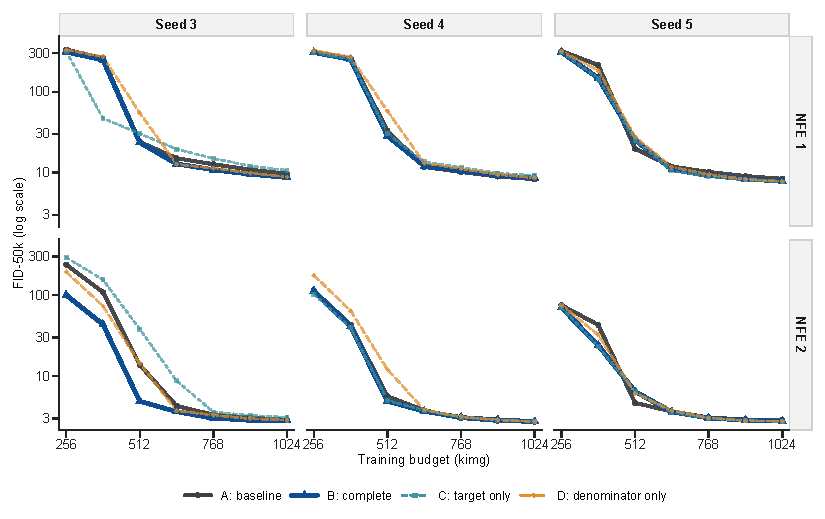
\includegraphics[width=\linewidth]
    {figures/figure2_seed_resolved_learning_curves.pdf}
  \caption{\textbf{Seed-resolved finite-budget learning trajectories.}
  Columns show formal training seeds 3--5 and rows show NFE1 and NFE2.
  Each curve contains the seven frozen budgets from 256 to 1024 kimg; every
  point is a FID-50k evaluation. Arms A and B are emphasized, while the
  target-assignment probe C and denominator-assignment probe D provide
  factorial context.
  The logarithmic FID axis exposes both the large early separations and the
  later contraction and crossings. Training seed is the independent unit;
  budgets and NFE readouts are repeated measurements, not additional
  replicates.}
  \label{fig:seed-resolved-curves}
\end{figure}

The assignment contrasts themselves are also budget dependent
(Figure~\ref{fig:factorial-contrast-curves}). Target, denominator, and
interaction trajectories can change sign even when their 256-kimg summaries
are directionally clear. This is the quality-level distinction between an
exact matched-state factorial identity and a factorial comparison after
separate training.

\begin{figure}[t]
  \centering
  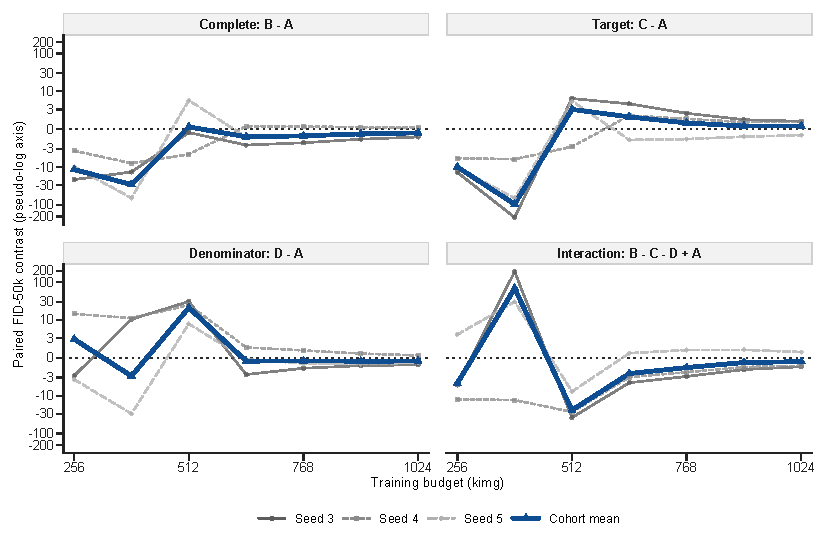
\includegraphics[width=\linewidth]
    {figures/figure4_budget_dependent_factorial_contrasts.pdf}
  \caption{\textbf{Budget-dependent NFE1 factorial contrasts.}
  Panels show the paired FID-50k contrasts $B-A$, $C-A$, $D-A$, and
  $B-C-D+A$ for each formal training seed and their descriptive cohort mean.
  Negative values favor the first named arm. The shared signed pseudo-log axis
  is linear near zero ($\sigma=1$) and logarithmic in both tails, allowing
  early large contrasts and later near-zero variation to remain visible on the
  same scale. The dotted line marks zero. All three seed trajectories are
  displayed; the blue mean is not treated as an additional replicate.}
  \label{fig:factorial-contrast-curves}
\end{figure}

\subsection{Secondary long-budget sensitivity}

At 1024 kimg, a post-preregistered five-seed sensitivity cohort has
descriptive mean minima in D under NFE1 and A under NFE2 for both FID and KID,
documenting descriptive sampler-readout variation without establishing a population
ranking (Appendix Table~\ref{tab:secondary-1024}).

\empnote{Figure 3: predefine log-FID AUC and time-to-quality only for the new
prospectively frozen cohort. Existing curves can illustrate these quantities
but must not be retroactively labeled confirmatory.}

\section{Why common-state identities do not determine trajectories}
\label{sec:stateful-trajectories}

Under Proposition~\ref{prop:sg-product-structure}'s conditions, the exact
identities in Section~\ref{sec:theory} determine the local interaction whenever
the cells are evaluated at one parameter value and under matched stochastic
inputs. Training instead evaluates each cell at its own evolving state, so the
common-state identities alone do not close the recursion for a factorial
contrast formed after the four arms are trained separately.

\begin{proposition}[Exact trajectory-feedback recursion]
\label{prop:trajectory-feedback}
Let $G_{X,k}(\theta)$ be arm $X\in\{A,B,C,D\}$'s one-sided minibatch
training field under the shared stochastic realization $\zeta_k$, and consider
plain SGD with $\eta_k\geq0$
\begin{equation}
  \theta_{X,k+1}=\theta_{X,k}-\eta_kG_{X,k}(\theta_{X,k}).
  \label{eq:shared-rng-sgd}
\end{equation}
Define the parameter factorial contrast and matched-state local interaction
\begin{align}
  \Psi_k&:=\theta_{B,k}-\theta_{C,k}-\theta_{D,k}+\theta_{A,k},
  \label{eq:parameter-factorial}\\
  I_k^{\mathrm{loc}}(\theta)
  &:=G_{B,k}(\theta)-G_{C,k}(\theta)
    -G_{D,k}(\theta)+G_{A,k}(\theta).
  \label{eq:matched-local-interaction}
\end{align}
Then
\begin{equation}
  \Psi_{k+1}=\Psi_k-\eta_k
  \left[I_k^{\mathrm{loc}}(\theta_{A,k})+R_k\right],
  \label{eq:exact-trajectory-feedback}
\end{equation}
where the state-divergence feedback is
\begin{align}
  R_k:={}&
  \left[G_{B,k}(\theta_{B,k})-G_{B,k}(\theta_{A,k})\right]
  \nonumber\\[-2pt]
  &-\left[G_{C,k}(\theta_{C,k})-G_{C,k}(\theta_{A,k})\right]
  \nonumber\\[-2pt]
  &-\left[G_{D,k}(\theta_{D,k})-G_{D,k}(\theta_{A,k})\right].
  \label{eq:state-divergence-feedback}
\end{align}
\end{proposition}

In the current unclipped constant-ratio setting,
$G_{B,k}(\theta)=sG_{C,k}(\theta)$ and
$G_{D,k}(\theta)=sG_{A,k}(\theta)$ at every matched state satisfying the
proposition's differentiability condition (or using the shared endpoint-wise
subgradient selection specified above), so
\begin{equation}
  I_k^{\mathrm{loc}}(\theta)
  =(s-1)\left[G_{C,k}(\theta)-G_{A,k}(\theta)\right].
  \label{eq:constant-s-local-interaction}
\end{equation}
Equation~\eqref{eq:exact-trajectory-feedback} separates this exactly known
local term from feedback created by state separation. Under Lipschitz training
fields, Appendix~\ref{app:trajectory-proof} bounds the feedback through the
A-centered arm separation; the recursion does not generally close in
$\Psi_k$ alone. This bound uses standard coupled-iterate stability reasoning
\citep{hardt2016train}. The recurrence delineates the implication boundary from
common-state identities to separately trained factorial contrasts. It does not
predict the sign or magnitude of FID contrasts and does not explain their
observed contraction with budget.

\claimnote{Use the recurrence only for the non-implication from matched-state
identities to separately trained factorial contrasts. The observed contraction
is empirical and currently lacks a theory-level mechanism claim.}

\paragraph{Two steps suffice for a nonzero separately trained factorial
contrast.}
This implication boundary already appears in an abstract one-dimensional
smooth lifted loss. Let
$D_\theta=\theta$, $T^1_{\bar\theta}=-1$,
$T^g_{\bar\theta}=-1-\bar\theta$,
$\varphi(e)=e^2/2$, and use weights $w_1=1,w_g=s$ with $s>0$, $s\neq1$.
Writing $G_X$ for the corresponding one-sided field, we have
\begin{equation}
  G_A=1+\theta,\quad G_C=1+2\theta,\quad
  G_D=s(1+\theta),\quad G_B=s(1+2\theta),
  \label{eq:two-step-vector-fields}
\end{equation}
and satisfy $G_B=sG_C$ and $G_D=sG_A$ for every $\theta$. At the common initial
state, $I_0^{\mathrm{loc}}(0)=0$. Starting all arms at zero and taking two
deterministic SGD steps of size $\eta>0$ nevertheless gives
\begin{equation}
  \Psi_1=0,
  \qquad
  \Psi_2=(s^2-1)\eta^2\neq0.
  \label{eq:two-step-nonadditivity}
\end{equation}
Thus exact common-state scaling identities, even when valid globally in
parameter space, do not force the separately trained parameter factorial
contrast to remain zero. The parameter-space contrast is a
non-representation-invariant algebraic witness of this implication boundary,
not a model of FID.

We also measured the realized target-endpoint component at arm-A states from
seeds 3--5 and 256--1024 kimg using eight fixed batches per state. The exact
denominator identities held to relative error below $8.3\times10^{-6}$. The
whole-model ratio
$\lVert G_B-sG_A\rVert_2/\lVert G_A\rVert_2$ was small but nonzero
($0.00174$--$0.00363$), with layerwise 90th percentiles of
$0.00396$--$0.00511$. Its 1024-minus-256 kimg change was negative for one seed
and positive for two, while the aligned NFE1 FID contrasts changed in magnitude
and sign without a corresponding monotone change in this ratio. The frozen-state
target-component magnitude therefore does not by itself account for the
budget-resolved quality curves.

A frozen-state RAdam factorial supports the bounded claim that accumulated
optimizer state can alter a next-update scalar relation; it does not identify
the cause of finite-training quality differences
(Appendix~\ref{app:evaluation-audit}). A held-out moment-transport preflight
failed its registered gate, so no continuation or endpoint evaluation was
launched (Appendix~\ref{app:evaluation-audit}).

\claimnote{Keep this section compact. PR65 is a next-update diagnostic and
PR66 is a NO-GO result. Neither is endpoint mechanism closure.}

\section{Discussion, generalization, and limitations}
\label{sec:discussion}

\paragraph{Common-state algebra versus finite-training outcomes.}
The exact target-by-weight identities specify what changes in one matched ECT
loss and one-sided training field. Proposition~\ref{prop:trajectory-feedback}
shows why those identities do not determine the factorial contrast formed after
four separate training trajectories. The budget-dependent contraction is an
empirical observation; the recurrence does not supply its mechanism.

\paragraph{Learning efficiency is the prospective target.}
The present curves motivate a primary estimand based on NFE1 log-FID
learning-curve area over fixed budgets, with time-to-FID thresholds as
secondary summaries. These estimands require a prospectively frozen, unseen
training-seed cohort. Existing seeds are used to establish and motivate the
trajectory hypothesis, not to claim held-out confirmation of a retrospectively
chosen AUC.

\paragraph{General weighting rules.}
Proposition~\ref{prop:sg-product-structure} covers any explicit weight held
constant during the one-sided derivative. It does not cover an undetached
residual-dependent or learned weight, whose derivative contributes an
additional term. A direct generalization test would compare the realized
weight ratio under the CIFAR-style inverse-gap rule with a gap-independent
weighting regime. The second-regime network audit remains pending.
Inverse-gap and gap-independent weighting regimes have both appeared in
consistency training \citep{geng2024consistency,silvestri2025vct}, making their
contrast a direct
test of the weight-ratio term rather than a new weighting proposal.

\paragraph{What the $q$-fixed design studies.}
The present factorial studies a controlled spacing
perturbation conditional on the $q=256$ curriculum. In the evaluated
single-stage regime, Equation~\eqref{eq:q-g-exact-reparameterization} shows that
the $g=1.10$ pair rule is exactly the fixed-$q_{\mathrm{eff}}$ rule at pair
construction. A deterministic pair/loss/training-field audit is required to
close implementation equivalence; until then we make no full-training
equivalence claim. The matched-$q$ design remains a control rather than an
independent mechanism.

\paragraph{Current limitations.}
The formal budget-resolved evidence contains three independent training seeds
in one CIFAR-10 ECT setting, complemented by five post-preregistration
secondary seeds. FID and KID share an Inception-based representation, and NFE1
and NFE2 produce different rankings. Each metric cell uses one 50k sample set,
so evaluator Monte Carlo variation is not estimated and small late-budget
rankings remain descriptive. The current evidence therefore supports
trajectory-dependent learning effects in this setting. Generalization across
architectures, datasets, weighting rules, and samplers remains untested.
A prospectively unseen cohort and a second weighting regime are the
highest-value extensions.

\section{Conclusion}
\label{sec:conclusion}

In the inverse-spacing ECT objective studied here, a controlled pair-spacing
change is an exact composite intervention: it changes both the detached target
endpoint and the explicit loss denominator.
Their one-sided training fields obey exact common-state scaling identities.
The trajectory-feedback recursion and two-step construction delineate why those
identities do not determine the parameter factorial contrast after separate
training. Controlled four-arm experiments document large early
quality differences, later contraction, and rankings that vary with seed and
sampling NFE. In the evaluated ECT runs, the pair-spacing intervention produced
finite-budget differences whose magnitudes and rankings varied with trajectory
and sampling readout, alongside its exact common-state intervention structure.

\subsection*{AI use statement}

Generative AI tools assisted with conceptual framing, formulation and revision
of mathematical claims, proof development and checking, hypothesis and
experimental-design feedback, implementation and testing of analysis/audit
code, result interpretation, literature search and summarization, translation,
manuscript organization and drafting, reference and LaTeX formatting, and
prose editing. They did not generate experimental measurements or synthetic
datasets used as evidence. The authors checked AI-assisted equations, proofs,
citations, code, and numerical transcriptions against primary sources and
repository records, and take responsibility for the final content.

\todo{All authors must review this required ICLR 2027 disclosure and add any
other reportable AI uses before submission.}

\subsection*{Ethics statement}

This work studies optimization behavior on a standard public image benchmark
and introduces no human-participant study or private dataset. The main risks
are scientific: overgeneralizing from a limited set of seeds or presenting
secondary analyses as confirmatory. We address these risks by reporting the
training seed as the independent unit, separating formal and secondary cohorts,
and preserving the stated claim ceilings.

\subsection*{Reproducibility statement}

The supplementary material records the four-arm intervention, seed and budget
matrix, frozen evaluation protocol, artifact-completeness audits, and the
assumptions behind the exact decomposition. The code and machine-readable
records will be provided through an anonymous supplementary artifact for
review.

\todo{Create and verify the anonymous artifact URL; do not link an
identity-revealing repository in the double-blind submission.}

\bibliography{OVERLEAF_ICLR2027_REFERENCES}
\bibliographystyle{iclr2027_conference}

\appendix

\section{Proof of ideal endpoint invariance}
\label{app:ideal-proof}

Fix $S\in\{S_1,S_2\}$, a supported $(\omega,t_0)$, and its legal schedule
sequence. The pointwise edge premise gives, for every $m$ before the anchor,
\begin{equation}
  F_S^\star(\gamma_\omega(t_m),t_m)
  =F_S^\star(\gamma_\omega(t_{m+1}),t_{m+1}).
\end{equation}
If the sequence reaches $t_\star$ after $M$ steps, repeated substitution gives
\begin{equation}
  F_S^\star(\gamma_\omega(t_0),t_0)
  =F_S^\star(\gamma_\omega(t_\star),t_\star)
  =b(\gamma_\omega(t_\star)).
\end{equation}
If $t_m\downarrow t_\star$, the same repeated substitution shows that the
left-hand side equals $F_S^\star(\gamma_\omega(t_m),t_m)$ for every $m$.
Continuity along the legal sequence and the common boundary condition give the
same limit. The right-hand side depends on the latent path and anchor, not on
the legal schedule or the choice of feasible ideal solution. Applying the
argument separately to $S_1$ and $S_2$ proves
Lemma~\ref{lem:ideal-endpoint-invariance} on their common reachable support.

For either formal stage-0 rule, write $h=1$ for the baseline and $h=g$ for the
enlarged spacing. Because $h n(t)/q<1$ in the audited unclipped regime, and
using $n(t)\geq1$,
\begin{equation}
  0<t_{m+1}
  =t_m\left(1-\frac{h n(t_m)}{q}\right)
  \leq\left(1-\frac{h}{q}\right)t_m.
\end{equation}
Thus $t_m\leq(1-h/q)^m t_0\rightarrow0$, establishing asymptotic anchor
reachability for both schedules. If a clamp is active, it reaches zero in one
step. If zero edge residual is inferred from a zero expected
positive-weight loss, the equality first holds almost everywhere; a pointwise
claim additionally requires the corresponding support-closure and continuity
conditions.

\section{Proof of the exact one-sided identities}
\label{app:sg-proof}

During the one-sided derivative, $w_r$, $T_{\bar\theta,r}$, and $\zeta$ are
fixed. The chain rule therefore gives
\begin{equation}
  \left.\nabla_\theta\widetilde\ell_{r,w}
  \right|_{\bar\theta=\theta}
  =w_rJ_t^\top\nabla\varphi(e_r)=w_rH_r,
\end{equation}
which proves Equation~\eqref{eq:sg-product-structure}. Setting
$\alpha=w_g/w_1$ and adding and subtracting the baseline-endpoint value and
field terms gives
Equations~\eqref{eq:general-loss-decomposition} and
\eqref{eq:general-weight-decomposition}. Substitution of
\begin{equation}
  G_A^{\mathrm{sg}}=w_1H_{r_1},\quad
  G_C^{\mathrm{sg}}=w_1H_{r_g},\quad
  G_D^{\mathrm{sg}}=w_gH_{r_1},\quad
  G_B^{\mathrm{sg}}=w_gH_{r_g}
\end{equation}
proves all factorial identities. In particular, the complete field change has
the two exact paths
\begin{align}
  G_B^{\mathrm{sg}}-G_A^{\mathrm{sg}}
  &=(w_g-w_1)H_{r_1}+w_g(H_{r_g}-H_{r_1}),\\
  &=w_1(H_{r_g}-H_{r_1})+(w_g-w_1)H_{r_g}.
\end{align}
The two decompositions have the same total. Their target components differ by
$I_G=(w_g-w_1)(H_{r_g}-H_{r_1})$, while their explicit-weight components differ
by the opposite amount. Hence neither path defines a unique component
attribution for the factorial contrast formed from separately trained quality
outcomes.

For $\varphi(e)=\lVert e\rVert_2$ at $e=0$, replace
$\nabla\varphi(e_r)$ by a selected $v_r\in\partial\lVert e_r\rVert_2$.
Using the same selection for repeated occurrences of endpoint $r$ under
different weights preserves $H_r=J_t^\top v_r$ and therefore every product and
factorial identity above. The selection is additional mathematical data; the
identities do not determine an implementation's zero-residual convention.

If $w_r$ is not held fixed, the chain rule contains the additional term
$(\Dsg w_r)\varphi(e_r)$. Likewise, if the endpoint is differentiated through,
its derivative contributes another term. These cases are outside
Proposition~\ref{prop:sg-product-structure}.

\section{Trajectory-feedback proof and finite-horizon bound}
\label{app:trajectory-proof}

Substituting Equation~\eqref{eq:shared-rng-sgd} into
Equation~\eqref{eq:parameter-factorial}, then adding and subtracting
$G_{B,k}(\theta_{A,k})$, $G_{C,k}(\theta_{A,k})$, and
$G_{D,k}(\theta_{A,k})$, gives Equations
\eqref{eq:exact-trajectory-feedback}--
\eqref{eq:state-divergence-feedback}.

For a finite-horizon bound, suppose every $G_{X,k}$ is
$L_{X,k}$-Lipschitz and define
\begin{align}
  D_k&:=\max_{X\in\{B,C,D\}}
    \lVert\theta_{X,k}-\theta_{A,k}\rVert_2,\\
  L_k&:=\max_{X\in\{A,B,C,D\}}L_{X,k},\\
  M_k&:=\max_{X\in\{B,C,D\}}
    \lVert G_{X,k}(\theta_{A,k})-G_{A,k}(\theta_{A,k})\rVert_2.
\end{align}
Adding and subtracting $G_{X,k}(\theta_{A,k})$ in each arm difference yields
\begin{equation}
  D_{k+1}\leq(1+\eta_kL_k)D_k+\eta_kM_k.
  \label{eq:diameter-recursion}
\end{equation}
Iterating this inequality gives the discrete Gr\"onwall bound
\begin{equation}
  D_k\leq
  D_0\prod_{\ell=0}^{k-1}(1+\eta_\ell L_\ell)
  +\sum_{j=0}^{k-1}\eta_jM_j
    \prod_{\ell=j+1}^{k-1}(1+\eta_\ell L_\ell).
  \label{eq:diameter-gronwall}
\end{equation}
Moreover,
\begin{equation}
  \lVert R_k\rVert_2
  \leq(L_{B,k}+L_{C,k}+L_{D,k})D_k
  \leq3L_kD_k.
\end{equation}
Consequently,
\begin{equation}
  \lVert\Psi_K\rVert_2
  \leq\lVert\Psi_0\rVert_2
  +\sum_{k=0}^{K-1}\eta_k
  \left[
    \lVert I_k^{\mathrm{loc}}(\theta_{A,k})\rVert_2+3L_kD_k
  \right].
  \label{eq:factorial-finite-horizon-bound}
\end{equation}
The displayed recursion is not closed in $\Psi_k$ alone; it also requires the
A-centered separation $D_k$. For the formal $c=0$ norm loss, this conditional
Lipschitz argument does not cover neighborhoods containing an exact zero
residual unless a regularized or consistently selected field is specified.

For the two-step construction, the first iterates are
$\theta_{A,1}=\theta_{C,1}=-\eta$ and
$\theta_{B,1}=\theta_{D,1}=-s\eta$. The second iterates are
\begin{align}
  \theta_{A,2}&=-2\eta+\eta^2,&
  \theta_{C,2}&=-2\eta+2\eta^2,\\
  \theta_{D,2}&=-2s\eta+s^2\eta^2,&
  \theta_{B,2}&=-2s\eta+2s^2\eta^2.
\end{align}
Substitution into Equation~\eqref{eq:parameter-factorial} gives
Equation~\eqref{eq:two-step-nonadditivity}.

\section{Evaluation and artifact audit summary}
\label{app:evaluation-audit}

\subsection{Frozen evaluation and trajectory provenance}

The formal factorial uses FP32 sampling with 50,000 generated examples per
job, sample seeds 0--49,999, and metric seed 20260730. KID and then FID are
computed from byte-identical retained generated Inception features against one
stated frozen CIFAR-10 reference. All NFE1 jobs precede all NFE2 jobs, and NFE2
uses the frozen intermediate time $0.821$. Across the contributing stages of
the carry-forward chain, PASS receipts bind each job's evaluator source,
checkpoint, detector/reference cache, generated features, and artifact tree by
SHA-256; failed jobs are not carried forward. Formal training and evaluation
used NVIDIA A100 80GB PCIe devices in the audited Python 3.10.12, PyTorch
2.2.0a0+81ea7a4, CUDA 12.3, and cuDNN 8.9.0.7 sandbox. Training used two
sequential GPU queues with deterministic algorithms, deterministic cuDNN,
\texttt{CUBLAS\_WORKSPACE\_CONFIG=:4096:8}, and cuDNN benchmarking disabled.
The evaluator maps generated outputs to uint8 as
$(127.5x+128)$ followed by clipping to $[0,255]$, applies no Python-side
resize, and requests pre-softmax features from the frozen
StyleGAN2-ADA Inception-2015-12-05 TorchScript detector; CIFAR-10 images enter
the same detector path as uint8 tensors.

Quality evaluation loads the EMA network stored in each selected snapshot.
The formal 256-kimg matrix admits every final arm checkpoint, with no preview
or intermediate-checkpoint selection, and evaluates it once per NFE. The
frozen KID definition averages 100 cubic-kernel estimates from independently
drawn, without-replacement real and generated subsets of size 1,000 using the
metric seed above. A cell is admitted only with a PASS receipt, clean
completion marker, and identical retained feature hash for KID and FID;
failed or missing cells are not imputed.

Two arm-C trajectories were resumed through the prevalidated exact-resume path
after a shared-memory infrastructure incident; the incident and resume evidence
are retained. At the common 256-kimg endpoint, seed-4 arm B records 1,991
accepted optimizer updates while arms A/C/D record 1,990, although all reach
2,000 attempts. We therefore do not overinterpret its small B--C difference.

\subsection{Formal complete-intervention contrast by budget}

\begin{table}[h]
  \caption{Budget-resolved NFE1 FID contrast for the complete intervention in
  formal seeds 3--5. Negative values favor arm B.}
  \label{tab:ba-curve}
  \centering
  \small
  \begin{tabular}{rrr}
    \toprule
    Budget (kimg) & Mean $B-A$ FID & Seeds favoring B \\
    \midrule
     256 & $-11.5408$ & $3/3$ \\
     384 & $-28.9498$ & $3/3$ \\
     512 & $ +0.2762$ & $2/3$ \\
     640 & $ -0.9574$ & $2/3$ \\
     768 & $ -0.8300$ & $2/3$ \\
     896 & $ -0.5755$ & $2/3$ \\
    1024 & $ -0.4502$ & $2/3$ \\
    \bottomrule
  \end{tabular}
\end{table}

\subsection{Secondary long-budget sensitivity}

Seeds 14--18 comprise 20 post-preregistration trajectories, six budgets from
384 to 1024 kimg, and 240 completed FID/KID-50k evaluation jobs. At 384 kimg,
the NFE1 FID means for A/B/C/D are $252.07/170.84/222.62/161.19$; at 640 kimg
they are $14.17/14.43/13.27/14.98$. Table~\ref{tab:secondary-1024} gives the
1024-kimg sensitivity summary.

\begin{table}[h]
  \caption{Secondary seeds 14--18 at 1024 kimg. Entries are five-seed cohort
  means and are sensitivity summaries, not additional formal replicates.}
  \label{tab:secondary-1024}
  \centering
  \small
  \begin{tabular}{crrrr}
    \toprule
    & \multicolumn{2}{c}{NFE1} & \multicolumn{2}{c}{NFE2} \\
    \cmidrule(lr){2-3}\cmidrule(lr){4-5}
    Arm & FID & KID & FID & KID \\
    \midrule
    A & 9.1761 & 0.005563 & \textbf{2.8768} & \textbf{0.001006} \\
    B & 8.9022 & 0.005506 & 2.9201 & 0.001114 \\
    C & 9.1882 & 0.005696 & 2.9472 & 0.001099 \\
    D & \textbf{8.6604} & \textbf{0.005362} & 2.8898 & 0.001025 \\
    \bottomrule
  \end{tabular}
\end{table}

\subsection{Frozen-state optimizer diagnostics}

For $U_0\neq0$, define the residual after best scalar alignment as
\begin{equation}
  \Ropt(U_1,U_0)
  :=\frac{\lVert U_1-c^\star U_0\rVert_2}{\lVert U_0\rVert_2},
  \qquad
  c^\star:=\frac{\langle U_1,U_0\rangle}{\lVert U_0\rVert_2^2}.
  \label{eq:optimizer-residual}
\end{equation}
Across seeds 3--5, the seed medians are $0.074$--$0.088$ for observed
gradients with real accumulated state, $0.467$--$0.491$ with reset state,
$0.049$--$0.077$ for an exact-scalar gradient under real state, and
$0.0006$--$0.0017$ when both the gradient and state are reduced to the fresh
scalar control. Thus the realized field residual and accumulated state
interact at the next-update level; this diagnostic does not identify an
endpoint-quality mechanism.

A separately frozen moment-transport proposal failed its held-out preflight:
all 12 rows increased rather than decreased the registered divergence. No
continuation training or FID/KID evaluation was launched.

\begin{table}[h]
  \caption{Status of the evidence used in the main text. A completed job means
  that the recorded evaluation and its required artifacts passed the
  corresponding repository audit.}
  \label{tab:evidence-status}
  \centering
  \small
  \begin{tabular}{p{0.25\linewidth}p{0.18\linewidth}p{0.44\linewidth}}
    \toprule
    Evidence block & Status & Scope \\
    \midrule
    Formal factorial & Complete &
    Seeds 3--5; four arms; 256 kimg; NFE1/2; 24 FID/KID-50k cells. \\
    Formal learning curves & Complete &
    Seeds 3--5; four arms; seven budgets; NFE1/2; 168 FID/KID-50k jobs. \\
    Secondary curves & Complete, secondary &
    Seeds 14--18; four arms; six budgets; NFE1/2; 240 FID/KID-50k jobs;
    complete selection/launch ledger remains to be packaged. \\
    RAdam virtual updates & Supporting only &
    Frozen-state next-update geometry; no endpoint causal claim. \\
    Moment transport & Scientific NO-GO &
    Held-out preflight worsened all 12 rows; no continuation training. \\
    Target-component audit & Complete, diagnostic &
    Seeds 3--5; arm A; four budgets; eight fixed batches per state; exact
    identity and artifact gates passed. \\
    Prospective cohort & Pending &
    Unseen seeds, frozen log-FID AUC, contraction, and time-to-quality. \\
    \bottomrule
  \end{tabular}
\end{table}

\ifshowcomments
\section{Collaboration checklist}
\label{app:collaboration-checklist}

% This checklist is deliberately visible only while comments are enabled.
\begin{enumerate}
  \item \todo{Obtain a second-author verification of all methods values copied
  from frozen records, then package the accepted evaluator/detector and
  reference-statistic digests.}
  \item \empnote{Figures owner: verify the existing seed-resolved learning
  curves and budget-dependent factorial contrasts after the final source-data
  freeze; preserve training seed as the unit.}
  \item \todo{Freeze the prospective cohort and primary AUC before launching
  any new training run.}
  \item \empnote{Target-component measurement is complete. Decide whether its
  seed-resolved budget diagnostic belongs in the main text or appendix; retain
  the non-mediation claim boundary.}
  \item \theorynote{The focused discretization, weighting, semigradient, and
  flow-map literature audit is complete. Re-run citation-status checks at the
  submission freeze, including the anonymous public ``Guide to Training
  Consistency Models'' metadata, and preserve the bounded novelty wording.}
  \item \todo{Disable comments, resolve every TODO/CHECK/CLAIM marker, compile
  with the official ICLR 2027 style, and confirm the 9-page main-text limit.}
\end{enumerate}
\fi

\end{document}
